\documentclass{article}
\usepackage{amssymb,amsmath,titling}
\usepackage{amssymb,mathtools,amsthm,amsmath}
\usepackage{float}
\usepackage{indentfirst}
\usepackage{listings}
\usepackage{xcolor}
\usepackage{hyperref}
\usepackage{subfig}
\usepackage{float}

\definecolor{codegreen}{rgb}{0,0.6,0}
\definecolor{codegray}{rgb}{0.5,0.5,0.5}
\definecolor{codepurple}{rgb}{0.58,0,0.82}
\definecolor{backcolour}{rgb}{0.95,0.95,0.92}

\lstdefinestyle{mystyle}{
    backgroundcolor=\color{backcolour},   
    commentstyle=\color{codegreen},
    keywordstyle=\color{magenta},
    numberstyle=\tiny\color{codegray},
    stringstyle=\color{codepurple},
    basicstyle=\ttfamily\footnotesize,
    breakatwhitespace=false,         
    breaklines=true,                 
    captionpos=b,                    
    keepspaces=true,                 
    numbers=left,                    
    numbersep=5pt,                  
    showspaces=false,                
    showstringspaces=false,
    showtabs=false,                  
    tabsize=2
}

\lstset{style=mystyle}
\title{ECS 171 Final Project Report}
\author{
  Sergio Santoyo\\
  \and
  Yuan Chang\\
  \and
  Cesar Guzman Avina\\
  \and
  Will Colbert\\
  \and
  Nathaniel Faxon\\
  \and
  Kanchan Kaur\\
  \and
  Parminder Singh\\
}
\date{May 2022}

\begin{document}

\begin{titlepage}
   \begin{center}
       \vspace*{4cm}
		\Large
       \textbf{Market Prediction Algorithm}

       \vspace{0.5cm}
        ECS 171: Machine Learning \\
        Group 7 Project Report
       \vspace{1.5cm}

       \textbf{Group member:}\\
Parminder Singh, Yuan Chang, Nathaniel Faxon, Cesar Guzman Avina, Kanchan Kaur, Will Colbert, Sergio Santoyo

       \vfill
       \href{https://github.com/nfax117/ECS171_Proj1}{Github Repository Link}
            
       \vspace{0.8cm}
            
   \end{center}
\end{titlepage}


\section{Introduction \& Background}
The stock market has evolved into a major component of our lives, as well as a reflection of the national and global economy. A stock represents ownership, or equity stake, in the company, and has served as a way for companies to raise capital. Additionally, the stock market enables individuals to grow their wealth, while holding companies accountable and keeping an eye on corporate regulation. The stock market impacts the overall economy, and therefore, impacts everyone, including non-investors. Because stock markets span all industries and sectors, it is a key factor in determining the state and cycle of the economy.

When the stock market crashes, there is a sudden decline of stock prices, which results in a loss of wealth, and are further driven by other economic factors and current events. A crash is propelled with investors selling in panic, dropping prices even more. This provides an opportunity for investors, as they can potentially buy stocks back at a much lower price.

Machine learning can be used to identify stock market and financial trends, typically done using the LSTM (Long Short-term Memory) model, support vector machines (SVM), artificial neural networks (ANN), and back propagation neural networks (BPNN). While machine learning can be used to predict stock prices and market crashes, this is a challenging problem. The stock market can be volatile, influenced by many factors, ranging from politics, unexpected events, psychological factors, a company’s performance, and so on. This dynamic nature of the stock market makes it difficult to accurately predict crashes and prices.

If a market prediction model is built to successfully predict a stock market crash, it can be beneficial to investors, while also giving a warning to companies and the general public. It can also be used in various fields/sectors. Here are a some examples: 

	\begin{itemize}
		\item Communication and Media
			\begin{itemize}
				\item Machine learning can process content on social media platforms from high-power individuals in the stock market, and predict the market in multiple scenarios.   
			\end{itemize}
		\item Finance
			\begin{itemize}
				\item The finance sector is one of the most hit sectors during a crash. Predicting the market could allow financial institutions to prepare for the consequences, like anticipating layoffs.
			\end{itemize}
		\item Leisure and Hospitality 
			\begin{itemize}
				\item Leisure and hospitality companies face significant economic struggles after a crash, making it difficult for smaller companies to remain in business. Predicting a market downfall would allow these companies to prepare for potential financial hardship, while also taking some action to keep customers, like offering discounted services that can be bought ahead of time, so customers will still participate after the crash. 
			\end{itemize}
	\end{itemize}
 
\section{Literature Review} 
Machine learning techniques have several applications to the problem of market prediction. This section includes examples and methods of related work done by researchers and analysts that have developed tools and techniques that predict stock market prices and assist in proper decision making.

Zhao et al. investigated the problem of financial time series prediction by utilizing Long Short-Term Memory (LSTM) neural network as a good predictor of static and dynamic prediction. Stock data are categorized as time-series multidimensional vectors. In many cases, the time-series problem can be tackled by the LSTM. Kai Chen al. presented that a LSTM based approach used for predicting stock movements would return a $13\%$ better yield in accuracy compared to others.\cite{LSTM} Additionally more similar to the work presented in this paper is the work done by Luca Di al. indicated that using LSTM and dropout over a 5-day prediction interval with only price series data produced a $72\%$ accuracy.\cite{Time-Weighted LSTM} To test the effectiveness of a time-weighted LSTM model, Zhao et al. conduct further studies on stock indexes such as the S\&P 500 and Dow Jones Industrial Index. It concluded that when altering the model to have the best parameters, the S\&P 500 returns $80.24\%$ accuracy while a single index such as Dow Jones Industrial Index returns an $83.21\%$.\cite{RNN} The accuracy of the models in these works, though not the highest result, can still be an effective indicator in predicting the market.

\section{Dataset Description and Exploratory Data Analysis} 
The dataset used throughout this project was supplied from Kaggle and Nasdaq. It provided us with 15032 rows which included the columns: closing, opening, low, and high prices as well as the volume, \% gain and loss, and price variation for S\&P 500. Data was taken from 1962 to 2021.\cite{SNP_Daily} 
Below is a description of each column:

The following are descriptions of the features for the observations in the data-set.

	\begin{itemize}
		\item Date - Trading date (YYYY-MM-DD)
		\item Open (\#) - Market opening price.
		\item High (\#) - Highest price during the trading day.
		\item Low (\#) - Lowest price during the trading day.
		\item Close (\#) - Price when the market closed for the day.
		\item Adjusted Close (\#) - Closing price after corporate actions are accounted for.
		\item Volume (\#) - Number of shares traded during the trading day.
%		\item \% Gain/Loss (\#) - Percentage Change between 2 consecutive closing prices. (Shows the gain/loss between 2 trading days)
%		\item Price Variation (\#) - Price fluctuation during the day. ((high-low)/Close)
		\item P/E ratio - Ratio of a company's share price to the company's earning per share.
		\item EPS - Monetary value of earning per outstanding share of common stock for a company.
	\end{itemize}
	
The dataset was selected because of the extensive range of dates it includes as well as the amount of details it has for each date. Overall there is a general trend upwards in the data relating to the Open, Close, High, Low, and Volume. As seen in the plots below:
\begin{figure}[h!]
\subfloat[Plot for open, close, high and low]{{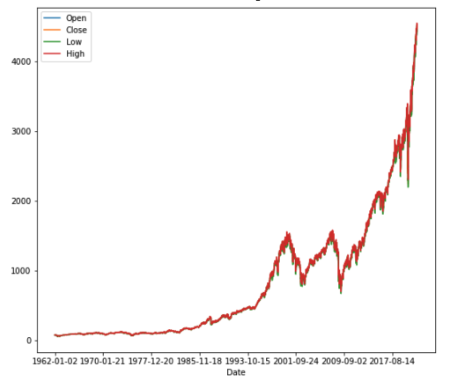
\includegraphics[scale=0.375]{p1.png} }}
    \qquad
    \subfloat[Plot for volume]{{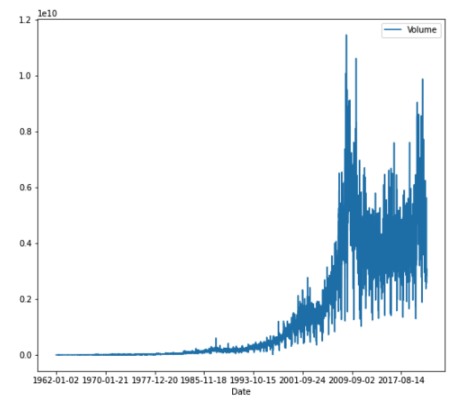
\includegraphics[scale=0.375]{p2.png} }}
    \caption{Example plots of the stock market's attributes}
    \label{fig:example}
\end{figure}


We thought that the PE ratio would be a stronger indicator of the market’s trend, and we used an additional S\&P 500 dataset that contains the monthly PE ratio\cite{SNP_PE_Monthly}, and it is from Nasdaq. In order to facilitate the PE ratio data, we extracted the attributes of the stock market for the first day of each month, and added the PE ratio column. This becomes the condensed datasets, which contain 717 data points.

PE ratio was excluded from the input attributes at the later stage, because it didn’t produce very accurate prediction models. After excluding it, we decided to use the daily stock dataset, which contains 15032 data points.

In order to process the input data set in the correct format for time series analysis, we chose 14 data points as our time step. Essentially, we are using the past 14 data point to predict a data point in the future, and repeat this process for the entire dataframe.
 
\section{Proposed Methodology} 

We will present here different models that we experimented with. They are linear regression, polynomial regression, univariate and multivariate time series analysis models. 

\subsection{Polynomial and Linear Regression}

As a basic starting step, we wanted to see if there were any relationships between a S\&P 500’s stock closing price and some other variable. After doing some research, we found that a good prediction of a stock's price comes from its P/E ratio multiplied by EPS. We made a dataset containing the value at the beginning of each month of the P/E ratio, EPS, P/E ratio multiplied by EPS, and the closing price for S\&P 500. To confirm variable relationships, we created a heat map(figure 3) with the variables as well as a pairplot(figure 2):

\begin{figure}[h!]
	\begin{center}
		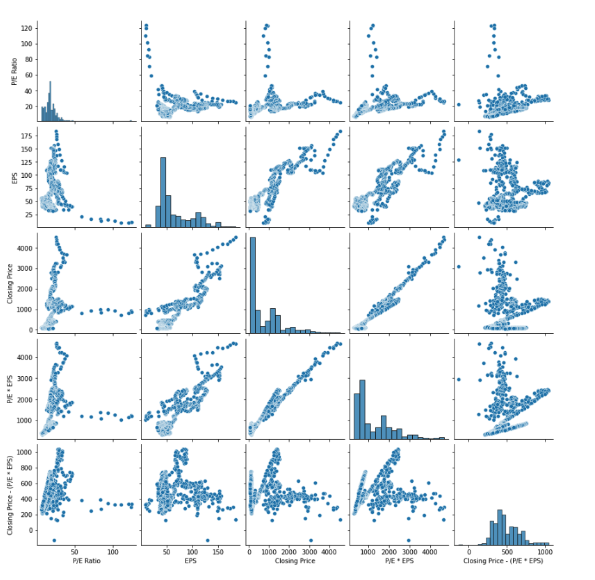
\includegraphics[scale=0.45]{p4.png}\caption{Heat map for the attributes}
	\end{center}
\end{figure}

\begin{figure}[H]
	\begin{center}
		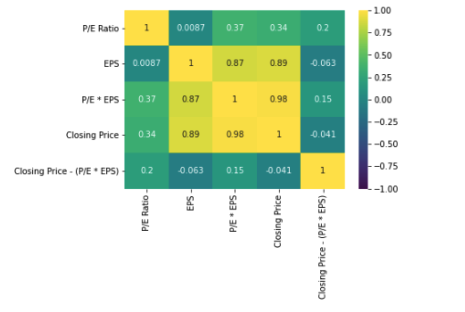
\includegraphics[scale=0.45]{p3.png}\caption{Heat map for the attributes}
	\end{center}
\end{figure}

As seen from the figures 2 and 3, Closing price and P/E * EPS seems to have a linear relationship. To test this, we created a linear regression model first to see the training MSE (Mean Squared Error) and how well a line visually fits the data. We also did a polynomial regression model with a degree of 2 just to see if the data had a polynomial relationship. For both these models, Sklearn’s Linear and Polynomial regression libraries were used and training and testing data was split by 80:20.

\begin{figure}[H]
\subfloat[Linear regression model plot]{{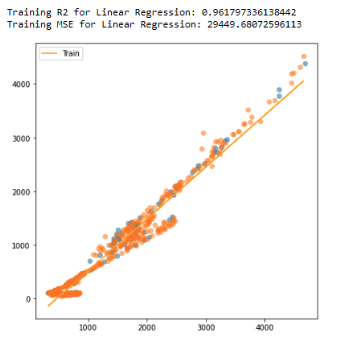
\includegraphics[scale=0.4]{p5.png} }}
    \qquad
    \subfloat[Polynomial Regression Degree = 2]{{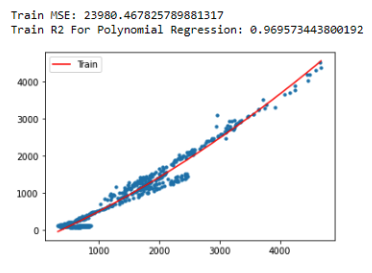
\includegraphics[scale=0.5]{p6.png} }}
    \caption{Plotted models}
    \label{fig:example}
\end{figure}
Based on the above results, there is a very high R2 score for both the linear and polynomial regressions which means that the line fits the data pretty well, thus high correlation between the two variables. There is a very high MSE, but this is due to how large the data values are and how many values there are in general. Though these models have helped show variable relationships and trends, we wanted to create more models that take into account more variables.

\subsection{Univariate}
In our next current implementation, we applied open, low, high, and volume features in addition to the closing price.
In our second version of our implementation it came to notice that our dataset is linked to time. So we approached it now using a Long Short Term Memory neural network. We started with a univariate LSTM model where the model predicted the closing price of the next day using the previous 50 days (time step), but the model failed to predict anything. We then chose to change the time step to 14 days, as this was the most used machine learning approach on the stock market. That result was looking promising, but we then realized that using previous closing prices to predict the next closing price is not a good feature. We decided to proceed in using more than one feature in our dataset to strengthen our model. 

\subsection{Multivariate}
In our most current implementation, we applied open, low, high, and volume features in addition to the closing price.

Since we were going to be predicting data points in the stock market, we knew that this would be a regression model problem. With this, we knew a neural network would need to be used to predict and find relationships between the data. Due to the fact that we are using multiple previous day values to predict the future stock price, we had to find a type of neural network that could utilize multiple sequences of data. After looking around we found that the Long Short Term Memory model was able to use multiple sequences, and then began to work with that type of model. We started with a univariate model of just using the Open price but realized that using more data attributes (Open, Close, High, Low, and Volume) in a multivariate model produced a more accurate model than univariate.

%While working on this model, we started to develop our website application so that our model could be interactive. We want to allow people to use our model and put in a date and get back an idea of the market price and whether or not there will be a crash. We use our pre-calculated data and upload it to a database to reference for when a date's data is requested.

\subsection{Time Series Model Configuration}
The exact configurations of the two time series models are shown below:
	\begin{itemize}
		\item Univariate model
			\begin{itemize}
				\item Using closing price alone
				\item 3 hidden layers
					\begin{itemize}
						\item  2 LSTM layer(one with return sequence, one without), 1 regular dense layer
						\item Units = [128,64,32,1]
						\item All using tanh as activation function, as default
					\end{itemize}
				\item First 2 layers employed dropout rate of 20\%
				\item Mini batch size tested: 4, 12, 16, 24, where size 24 achieved best accuracy.
			\end{itemize}
		\item Multivariate model
			\begin{itemize}
				\item Using [Open, Low, High, Volume, Closing price] as input attributes
				\item 3 hidden layers
					\begin{itemize}
						\item  2 LSTM layer(one with return sequence, one without), 1 regular dense layer
						\item Units = [64,64,32,1]
						\item All using tanh as activation function, as default
					\end{itemize}
				\item First 2 layers employed dropout rate of 20\%
				\item Mini batch size tested: 24 and 36, where size 36 achieved best accuracy.
			\end{itemize}
	\end{itemize}
\textit{Note: time series models that were trained from the condensed data set used time step of 14, where the models trained with full data set used time step of 45.}
%While working on this model, we started to develop our website application so that our model could be interactive. We want to allow people to use our model and put in a date and get back an idea of the market price and whether or not there will be a crash. We use our pre-built and uploaded database to reference the data for the date that is requested.


\section{Experimental Results} 

Since the prediction model we are building is essentially a regression model, we are using MSE and R2 score as the main evaluation metrics to compare different performing models. 

The experimental results for the linear and polynomial regression models were shown in the previous section, this section will be devoted to demonstrate the performance of the time series analysis models.

\subsection{Predicted Price Plots}

In order to visualize the performance of each time series model, we plotted the entire predicted price against the actual price. Note that the condensed model plots are plotting monthly, whereas the full models are plotting daily.\\

Below are the plots for the models that were trained using the condensed dataset, where it is spanning from January of 1962 to September of 2021, and the data is recorded monthly.

\begin{figure}[H]
\subfloat[Condensed Univariate]{{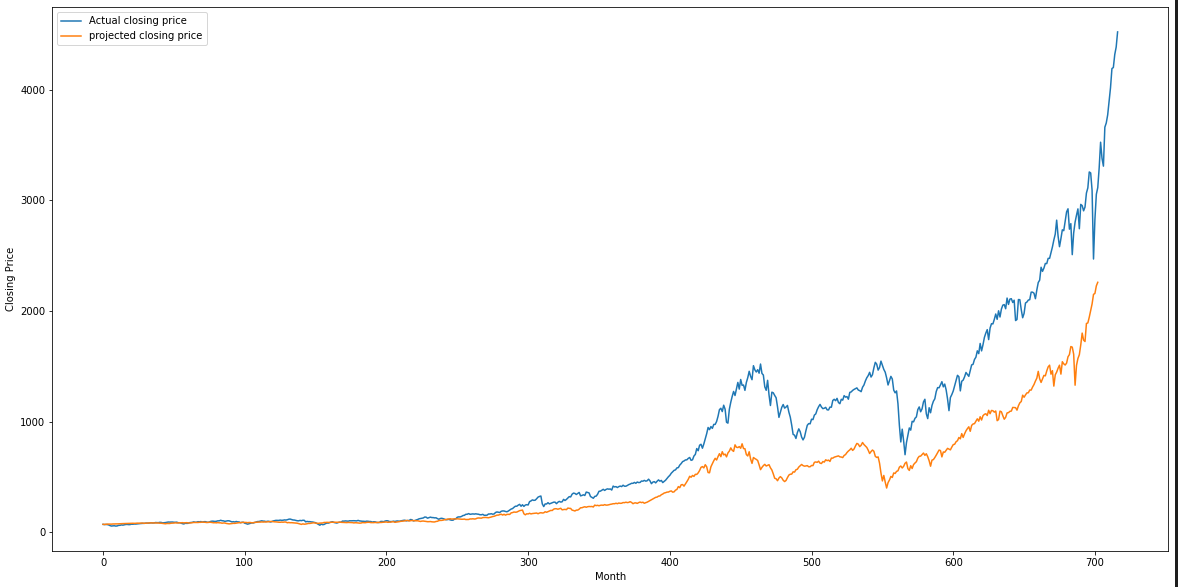
\includegraphics[scale=0.3]{p7.png} }}
    \qquad
    \subfloat[Condensed Multivariate]{{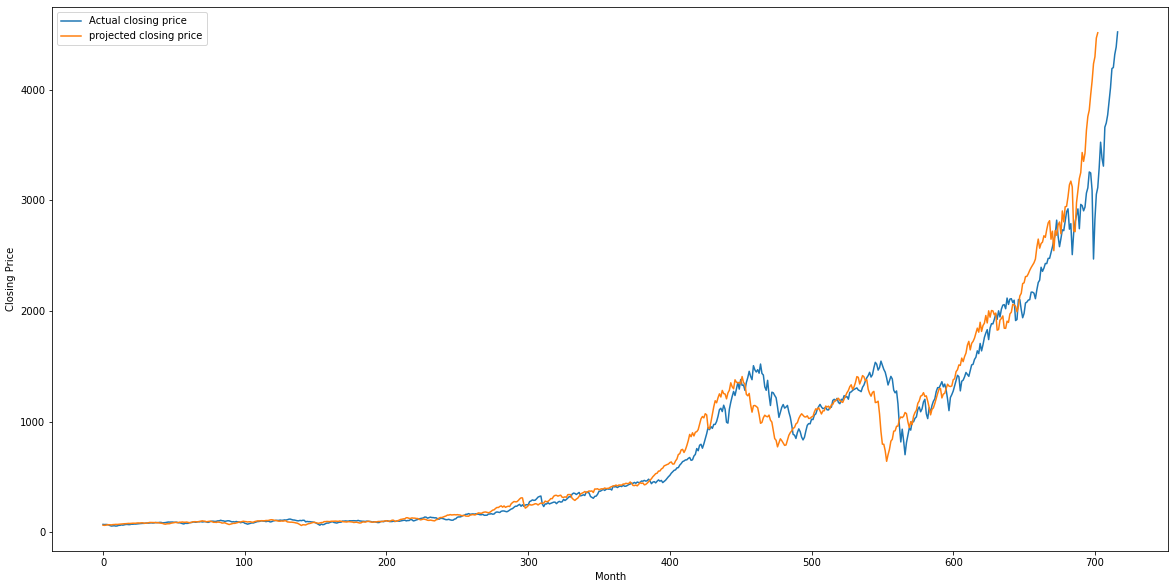
\includegraphics[scale=0.3]{p8.png} }}
    \caption{Condensed plots}
    \label{fig:example}
\end{figure}

The next two graphs plot the predicted price using the models trained from the full dataset. The full dataset contains daily recordings of the stock market since January $2^{\text{nd}}$ 1962 till September $17^{\text{th}}$ 2021.

\begin{figure}[H]
\subfloat[Full Univariate]{{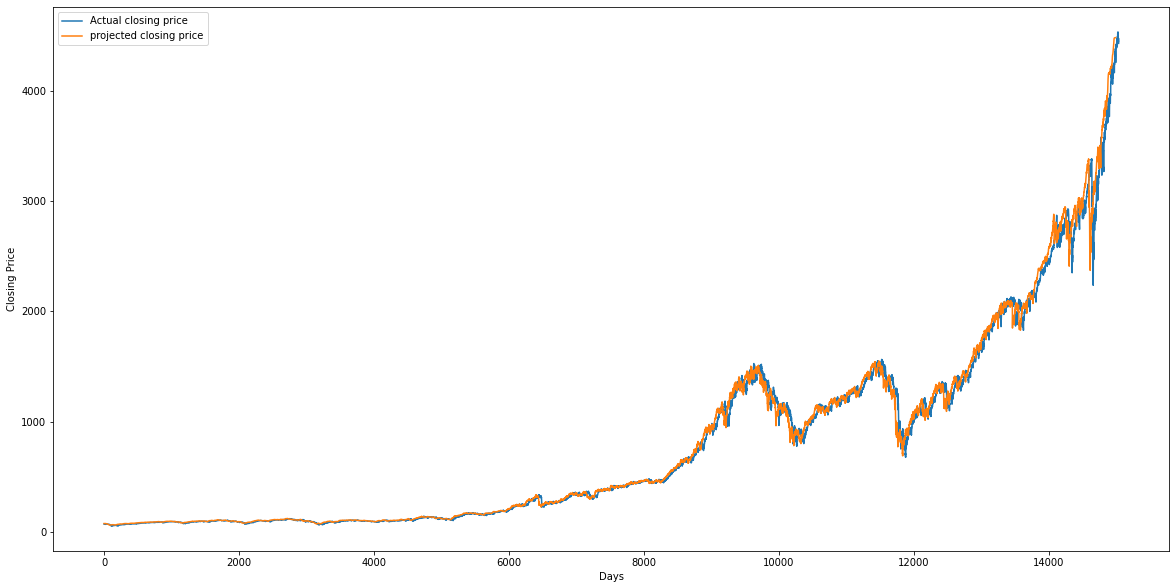
\includegraphics[scale=0.3]{p9.png} }}
    \qquad
    \subfloat[Full Multivariate]{{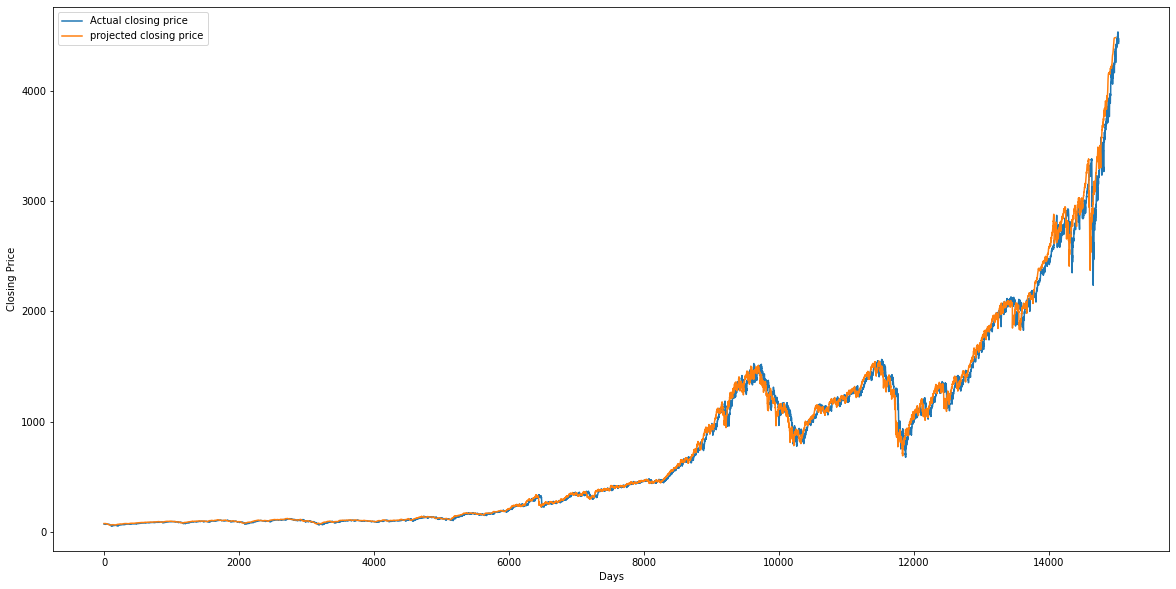
\includegraphics[scale=0.3]{p10.png} }}
    \caption{Full plots}
    \label{fig:example}
\end{figure}

\subsection{MSE \& R2 scores}
We calculated the MSE and R2 score for all of the time series models. There was a sharp decrease of MSE and an overall increase of R2 score when the dataset increased from condensed to full.

\begin{figure}[H]
	\begin{center}
		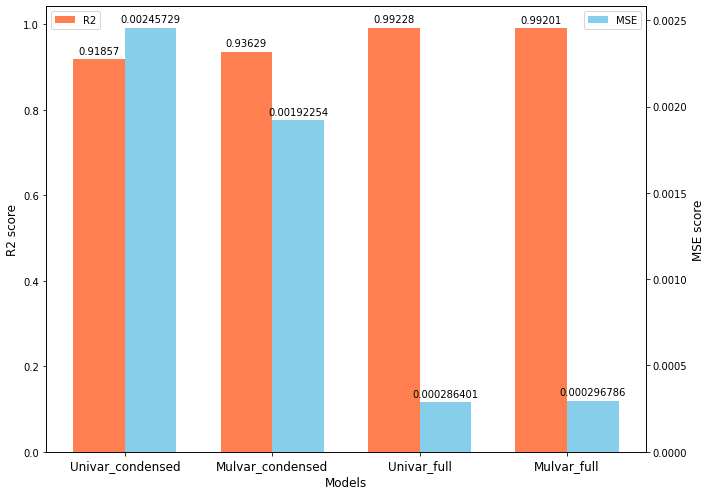
\includegraphics[scale=0.45]{p11.png}\caption{MSE and R2 scores of the time series models}
	\end{center}
\end{figure}

We also noticed that the highest R2 score and the lowest MSE were both recorded on the univariate model that was trained using the full dataset. This made sense as the univariate model was using closing price's history to predict future closing price. The multivariate model had attributes such as volume that might negatively impact the performance, since volume has weaker correlation to closing price compared to other attributes.  

\section{Conclusion and Evaluation} 
Using the datasets from Kaggle, which contained daily data about the open price, high price, low price, and closing price, volume, \% gain/loss, P/E ratio. We initially started with a linear and polynomial regression model, but we realized that the most optimal were the univariate and multivariate models. The best performance came from the univariate model of LSTM.\\

Our models were based strictly on numerical data, all the data in the dataset are taking in real world events in them. Our model cannot predict real world events in which stock market prices would make sporadic movements. So therefore, our model will not be able to capture any spikes in the stock price accurately.\\

For software implementation, we created two websites to display our data. The first one was used to display the project as a whole and the other to interact with the data. The interactive site utilized Flask, a web framework for developing web applications using python. After training our model, we saved the weights as well as the model architecture to use for the website. The backend code, loads and compiles the model, gets the input data from the user and uses it to predict the closing price of either 2021-09-18 (if user chooses not to give any data).\\

One of the conclusions we arrived at the end of this research project is that it is nearly impossible to predict the stock market’s closing price. In the real world, the stock market is volatile, dynamic and unpredictable. Thus, we can discuss the model’s improvements in two ways. First, since the models we produced were essentially models of the stock market of its current form, one potential improvement would be to increase the accuracy of our model. Ultimately to allow our model to mimic the stock market, at least till today. We could always increase the model’s performance through tuning the hyperparameters. In the interest of time, we only tuned the time step, number of nodes in each layer and the mini-batch size. Other than those, there are parameters such as the number of layers, activation function, regularization techniques we can try to improve the model. Furthermore, another direction to improve the model is to add additional attributes that reflect the population’s confidence level about the stock market. These kinds of attributes would be hard to quantify and produce, which may require their own machine learning models as well. Since the stock market’s closing price can be greatly influenced by people’s attitude, it would be an excellent addition to our time series model. 	


\begin{thebibliography}{9}
\bibitem{LSTM}
K. Chen, Y. Zhou and F. Dai, "A LSTM-based method for stock returns prediction: A case study of China stock market," 2015 IEEE International Conference on Big Data (Big Data), 2015, pp. 2823-2824, doi: 10.1109/BigData.2015.7364089.

\bibitem{Time-Weighted LSTM}
Di Persio, Luca, and Oleksandr Honchar. "Recurrent neural networks approach to the financial forecast of Google assets." International journal of Mathematics and Computers in simulation 11 (2017): 7-13.

\bibitem{RNN}
Z. Zhao, R. Rao, S. Tu and J. Shi, "Time-Weighted LSTM Model with Redefined Labeling for Stock Trend Prediction," 2017 IEEE 29th International Conference on Tools with Artificial Intelligence (ICTAI), 2017, pp. 1210-1217, doi: 10.1109/ICTAI.2017.00184.

\bibitem{SNP_Daily}
Myungchan Kim, "S\&P 500 Daily Data (1927-12-30 to 2021-09-19)," Yahoo Finance, url: https://www.kaggle.com/datasets/myungchankim/sp-500-daily-data-19281230-to-20210919/metadata.

\bibitem{SNP_PE_Monthly}
Nasdaq Data Link, "S\&P 500 PE Ratio by Month," Yahoo Finance, Data Link Code: MULTPL/SP500\_PE\_RATIO\_MONTH, url: https://data.nasdaq.com/data/MULTPL/SP500\_PE\_RATIO\_MONTH.

\end{thebibliography}
\end{document}








